%
%     hw9_bbordwell.tex
%     Baylee Bordwell (baylee.bordwell@colorado.edu)
%     Based on the template by Benjamin Brown (bpbrown@colorado.edu)
%     Aug 27, 2014
%
%     Problem set 9 for ASTR/ATOC 5540, Mathematical Methods, taught at
%     University of Colorado, Boulder, Fall 2014.
%
%

\documentclass[10pt, preprint]{aastex}
% formatting based on 2014 NASA ATP proposal with Jeff Oishi

%%%%%%begin preamble
\usepackage[hmargin=1in, vmargin=1in]{geometry} % Margins
\usepackage{hyperref}
\usepackage{url}
\usepackage{times}
\usepackage{natbib}
\usepackage{graphicx}
\usepackage{amsmath}
\usepackage{amsfonts}
\usepackage{amssymb}
\usepackage{pdfpages}
\usepackage{import}
% for code import
\usepackage{listings}
\usepackage{color}
\usepackage{ragged2e}

\hypersetup{
     colorlinks   = true,
     citecolor     = gray,
     urlcolor       = blue
}

%% headers
\usepackage{fancyhdr}
\pagestyle{fancy}
\lhead{ASTR/ATOC 5540}
\chead{}
\rhead{name: Baylee Bordwell}
\lfoot{Problem Set 9}
\cfoot{\thepage}
\rfoot{Fall 2014}
% no hline under header
\renewcommand{\headrulewidth}{0pt}

\newcommand{\sol}{\ensuremath{\odot}}

% make lists compact
\usepackage{enumitem}
%\setlist{nosep}

%%%%%%end preamble


\begin{document}
\section*{Problem Set 9: Dedalus and doubly-diffusive convection (a 2-D PDE)}
\begin{enumerate}
\setcounter{enumi}{-1}
\item Through dangers untold and hardships unnumbered...installed.

\item And it works! (as long as its own version of matplotlib is not used...)
\begin{figure}[!ht]
  \centering
  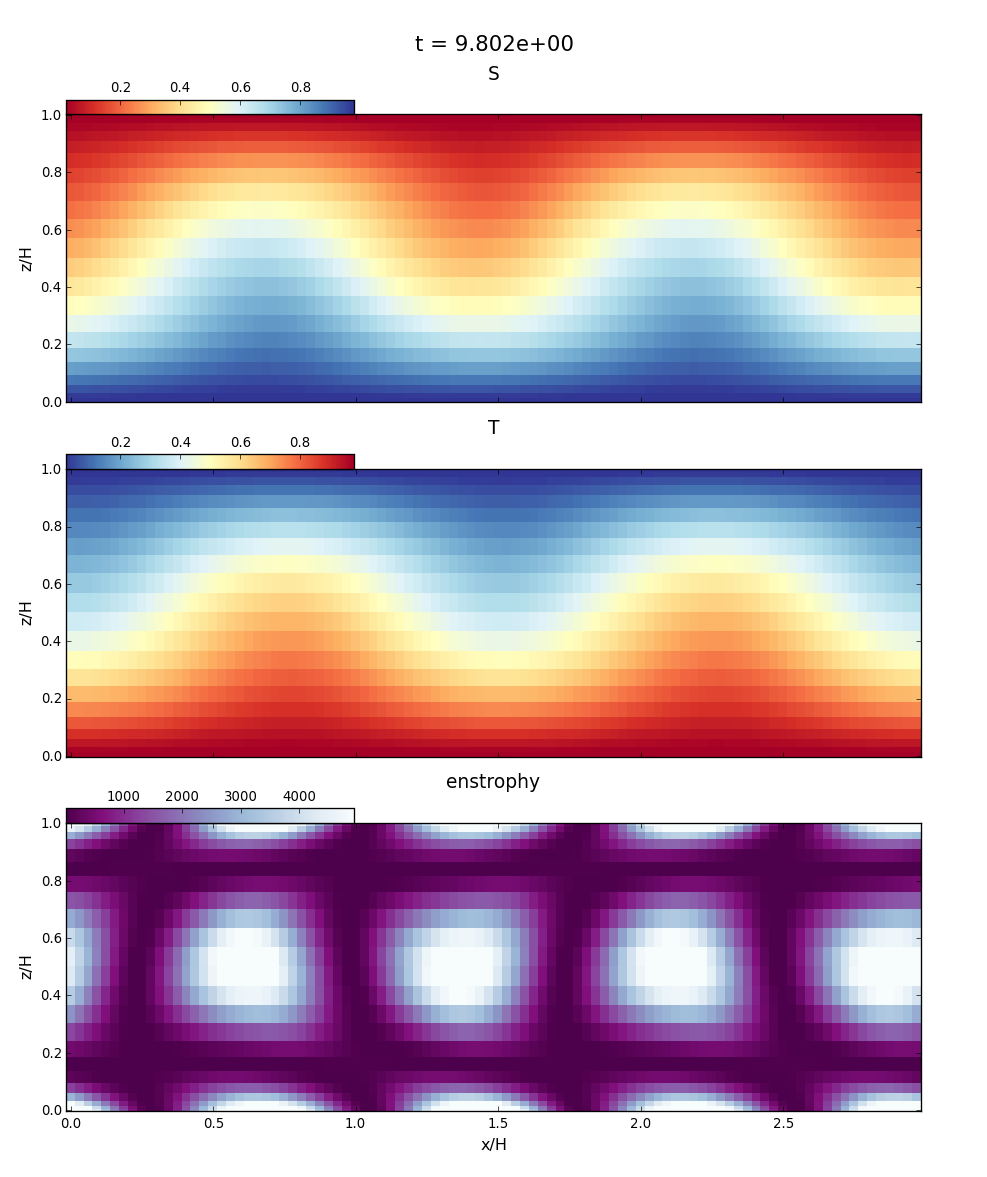
\includegraphics[width=2in]{TS/snapshot_000190.png}
\end{figure}

\item These are travelling waves, as the following images show.
\begin{figure}[!ht]
\minipage{0.32\textwidth}
  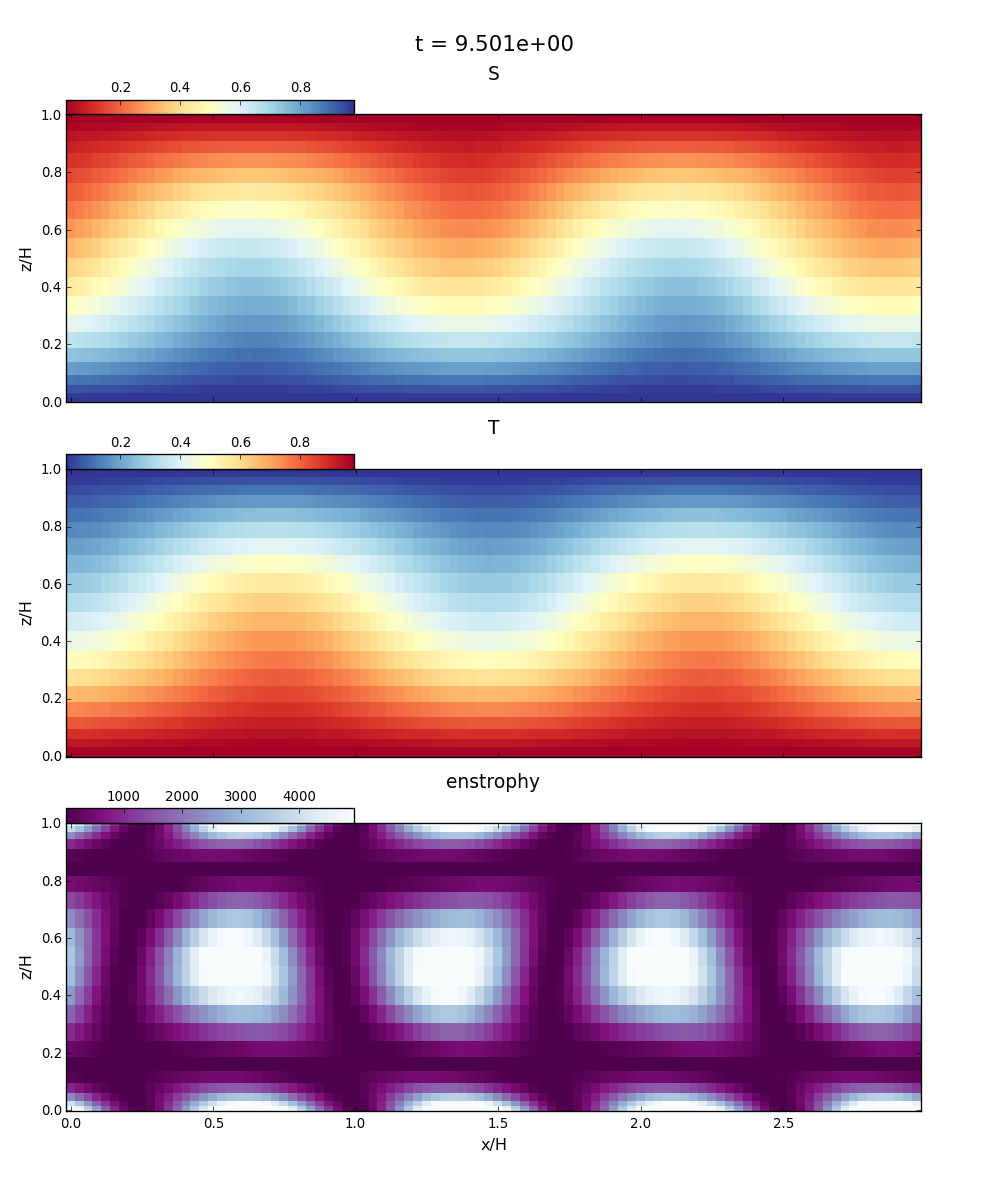
\includegraphics[width=2in]{TS/snapshot_000184.png}
\endminipage\hfill
\minipage{0.32\textwidth}
  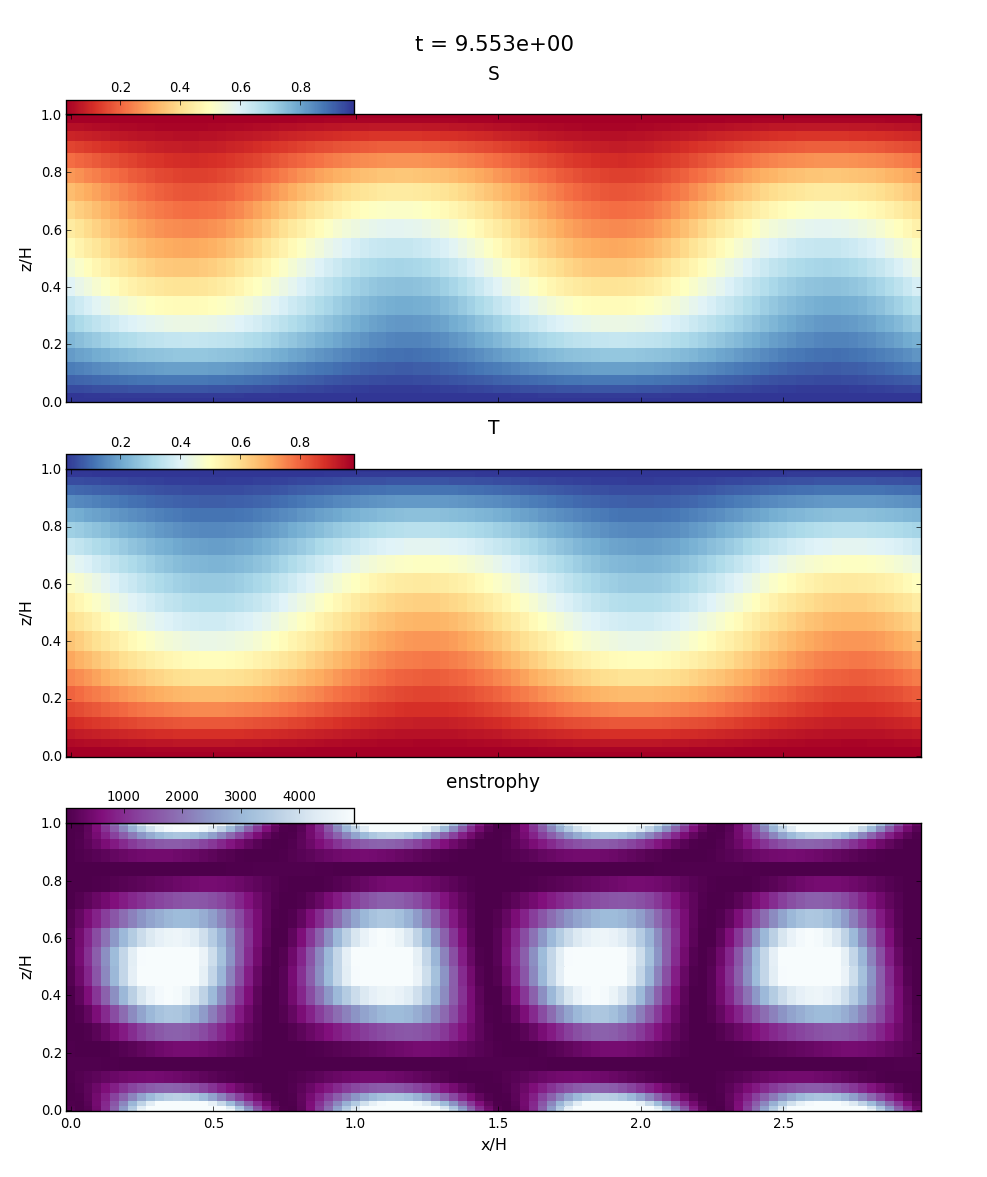
\includegraphics[width=2in]{TS/snapshot_000185.png}
\endminipage\hfill
\minipage{0.32\textwidth}
  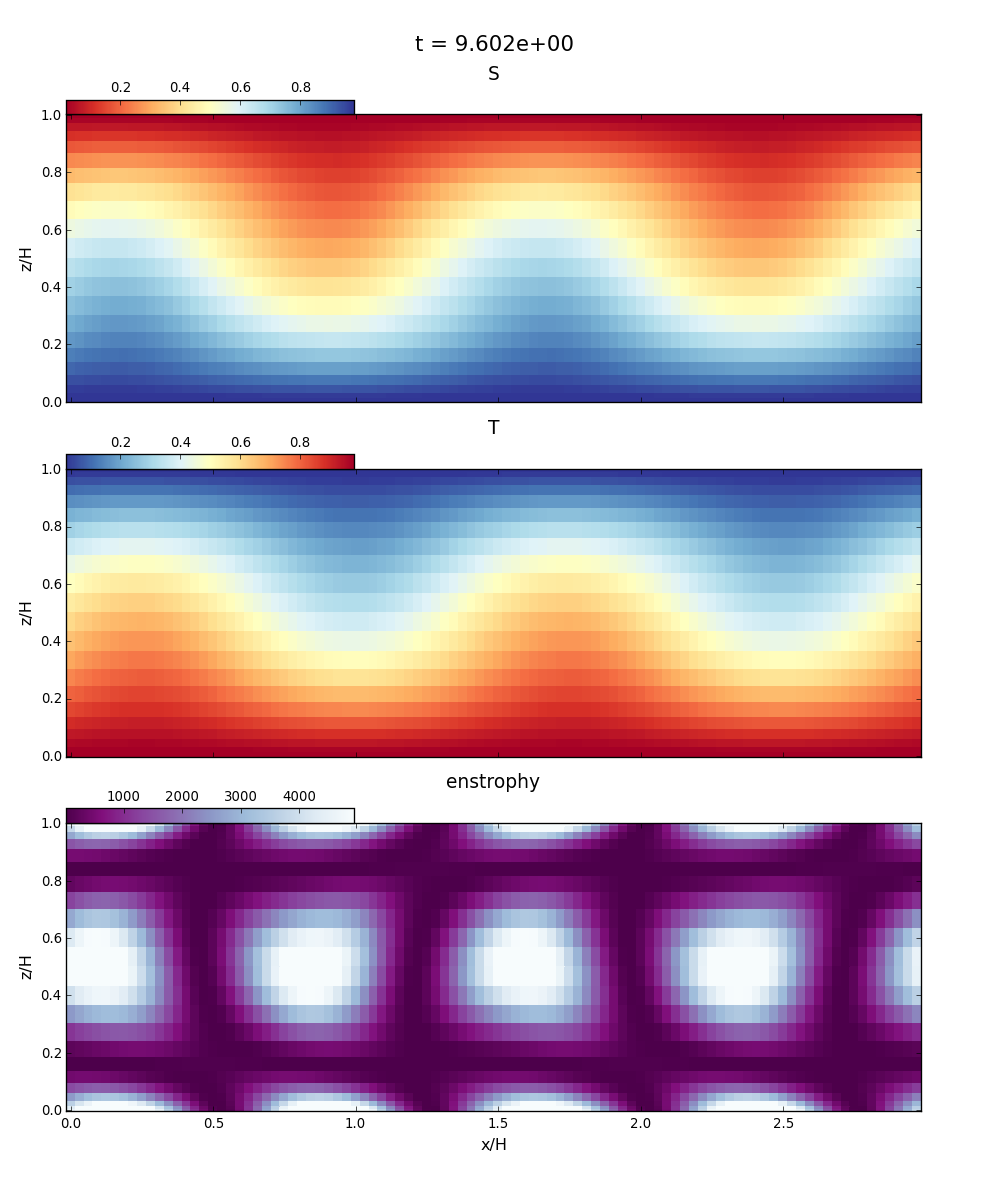
\includegraphics[width=2in]{TS/snapshot_000186.png}
\endminipage\hfill
\end{figure}

\item
\begin{table}[!ht]
  \centering
  \footnotesize
  \begin{tabular}{cl} \hline
    {\bf Equation} & {\bf Implementation} \\ \hline
    (1) & \verb|1/Pr*dt(w)  - (dx(dx(w)) + dz(w_z)) - Ra_T*T + Ra_S*S + dz(P) = -1/Pr*(u*dx(w) + w*w_z)| \\
    & \verb|1/Pr*dt(u)  - (dx(dx(u)) + dz(u_z)) + dx(P) = -1/Pr*(u*dx(u) + w*u_z)| \\
    (2) & \verb|dx(u) + w_z = 0| \\
    (3) & \verb|dt(T) - (dx(dx(T)) + dz(T_z)) = -u*dx(T) - w*T_z| \\
    (4) & \verb|dt(S) - Lewis*(dx(dx(S)) + dz(S_z)) = -u*dx(S) - w*S_z| \\
    \hline
    {\bf Implementation of} & {\bf Translation \hfill (in words)}\\ \hline
    (1) & $\frac{1}{Pr}\frac{\partial w}{\partial t} - \nabla^2 w\hat{z} - (Ra_TT-Ra_SS)\hat{z} 
    +\frac{\partial P}{\partial z} = -\frac{1}{Pr}\mathbf{u}\cdot \nabla w$ \hfill  $\hat{z}$ component of (1)\\
    & velocity current (in z), diffusion of velocity, buoyancy/sinking, pressure flux, advection of velocity \\
     & $\frac{1}{Pr}\frac{\partial u}{\partial t} - \nabla^2 u\hat{x} 
    +\frac{\partial P}{\partial x} = -\frac{1}{Pr}\mathbf{u}\cdot \nabla u$ \hfill  $\hat{x}$ component of (1)\\
    & velocity current (in x), diffusion of velocity, pressure flux, advection of velocity \\
    (2) & $\frac{\partial u}{\partial x} +\frac{\partial w}{\partial z} = 0$ \hfill the gradient of u, which = 0\\
    & outward flux of velocity is 0\\

    (3) & $ \frac{\partial T}{\partial t} -\nabla^2T = -\mathbf{u}\cdot \nabla T$ \hfill (I condensed the Laplacians and gradients in all of these...but I think that still IDs each term ok)\\
    & temperature current, temperature diffusion, temperature advection \\

    (4) & $ \frac{\partial S}{\partial t} - \tau\nabla^2S = -\mathbf{u}\cdot \nabla S$ \\
    & solute current, solute diffusion, solute advection \\
  \end{tabular}
  \caption{Translation of equations of thermosolutal convection from TS.py code. \label{tab1} \centering}
\end{table}
\begin{itemize}
\item The implementation of the equations of thermosolutal convection are detailed in Table \ref{tab1}. 
\item The role of equations like $dz(w)-w_z = 0$ are to keep the problem first order. As the x differentiation is essentially just a scalar multiplication, it is not necessary to do this for the x-derivatives, but for z-derivatives this simplifies the problem.
\item The equations are correctly implemented.
\item The boundary conditions are ([bottom,top]): \newline
$S=[1,0]$, $T=[1,0]$, $u=[0,0]$, $w=[0,0]$, 
  $\frac{\partial w}{\partial x}|_{\text{bottom}} \ne 0$, $P(\text{bottom}) = 0$,
  $\frac{\partial P}{\partial x}|_{\text{bottom}} = 0$
\end{itemize}

\item See Table \ref{tab2}. In \verb|equations.py|, the linear terms are all grouped on the left-hand side of the equation, and the non-linear terms are all on the right.
\begin{table}[!ht]
\centering
\footnotesize
\begin{tabular}{ccc} \hline
{\bf Equation} & {\bf Linear} & {\bf Nonlinear} \\ \hline
(1) & $\frac{1}{Pr}\frac{\partial \mathbf{u}}{\partial t}$,
$\nabla^2 \mathbf{u}$, $(Ra_TT-Ra_SS)\hat{z}$,$\nabla P$ & 
$\mathbf{u}\cdot\nabla\mathbf{u}$ \\ 
& \verb|1/Pr*dt(w), dx(dx(w)), dz(w_z), -Ra_T*T, Ra_S*S, dz(P)| & 
\verb|-1/Pr*u*dx(w), -1/Pr*w*w_z| \\
& \verb|1/Pr*dt(u), dx(dx(u)), dz(u_z), dx(P)| & 
\verb|-1/Pr*u*dx(u), -1/Pr* w*u_z| \\
(2) & $\nabla\cdot\mathbf{u}$ & - \\
& \verb|dx(u), w_z| & - \\
(3) & $\frac{\partial T}{\partial t}$, $\nabla^2T$ & $\mathbf{u}\cdot\nabla T$ \\
& \verb|dt(T), dx(dx(T)), dz(T_z))| & \verb|-u*dx(T), - w*T_z| \\
(4) & $\frac{\partial S}{\partial t}$, $\tau\nabla^2S$ & $\mathbf{u}\cdot\nabla S$\\
& \verb|dt(S), dx(dx(S)), dz(S_z))| & \verb|-u*dx(S), -w*S_z| \\
\end{tabular}
\caption{The linear and nonlinear breakdown of the equations in both raw and implemented form.\label{tab2} \centering}
\end{table}

\item T is destabilizing, while S is stabilizing. To change their relative roles I would set their boundary conditions to $[0,1]$, rather than $[1,0]$.
\end{enumerate}
Code used in this assignment:
%
%     hw9_code.tex
%     Baylee Bordwell
%     Template from: Benjamin Brown (bpbrown@colorado.edu)
%     Aug 27, 2014
%
%     Problem set 9 for ASTR/ATOC 5540, Mathematical Methods, taught at
%     University of Colorado, Boulder, Fall 2014.
%
%     Python code importing block.
%


\definecolor{codegreen}{rgb}{0,0.6,0}
\definecolor{codegray}{rgb}{0.5,0.5,0.5}
\definecolor{codepurple}{rgb}{0.58,0,0.82}
\definecolor{backcolour}{rgb}{0.95,0.95,0.92}
 
\lstdefinestyle{mystyle}{
    backgroundcolor=\color{backcolour},   
    commentstyle=\color{codegreen},
    keywordstyle=\color{magenta},
    numberstyle=\tiny\color{codegray},
    stringstyle=\color{codepurple},
    basicstyle=\footnotesize,
    breakatwhitespace=false,         
    breaklines=true,                 
    captionpos=b,                    
    keepspaces=true,                 
    numbers=left,                    
    numbersep=5pt,                  
    showspaces=false,                
    showstringspaces=false,
    showtabs=false,                  
    tabsize=2
}

\lstset{style=mystyle}


\lstinputlisting[language=Bash]{hw9_bbordwell.sh}


\end{document}
